% Options for packages loaded elsewhere
\PassOptionsToPackage{unicode}{hyperref}
\PassOptionsToPackage{hyphens}{url}
\PassOptionsToPackage{dvipsnames,svgnames*,x11names*}{xcolor}
%
\documentclass[
]{article}
\usepackage{lmodern}
\usepackage{amssymb,amsmath}
\usepackage{ifxetex,ifluatex}
\ifnum 0\ifxetex 1\fi\ifluatex 1\fi=0 % if pdftex
  \usepackage[T1]{fontenc}
  \usepackage[utf8]{inputenc}
  \usepackage{textcomp} % provide euro and other symbols
\else % if luatex or xetex
  \usepackage{unicode-math}
  \defaultfontfeatures{Scale=MatchLowercase}
  \defaultfontfeatures[\rmfamily]{Ligatures=TeX,Scale=1}
\fi
% Use upquote if available, for straight quotes in verbatim environments
\IfFileExists{upquote.sty}{\usepackage{upquote}}{}
\IfFileExists{microtype.sty}{% use microtype if available
  \usepackage[]{microtype}
  \UseMicrotypeSet[protrusion]{basicmath} % disable protrusion for tt fonts
}{}
\makeatletter
\@ifundefined{KOMAClassName}{% if non-KOMA class
  \IfFileExists{parskip.sty}{%
    \usepackage{parskip}
  }{% else
    \setlength{\parindent}{0pt}
    \setlength{\parskip}{6pt plus 2pt minus 1pt}}
}{% if KOMA class
  \KOMAoptions{parskip=half}}
\makeatother
\usepackage{xcolor}
\IfFileExists{xurl.sty}{\usepackage{xurl}}{} % add URL line breaks if available
\IfFileExists{bookmark.sty}{\usepackage{bookmark}}{\usepackage{hyperref}}
\hypersetup{
  pdftitle={MSU Graduate Spatial Ecology Lab 3},
  pdfauthor={Phoebe Zarnetske; plz@msu.edu},
  colorlinks=true,
  linkcolor=Maroon,
  filecolor=Maroon,
  citecolor=Blue,
  urlcolor=blue,
  pdfcreator={LaTeX via pandoc}}
\urlstyle{same} % disable monospaced font for URLs
\usepackage[margin=1in]{geometry}
\usepackage{color}
\usepackage{fancyvrb}
\newcommand{\VerbBar}{|}
\newcommand{\VERB}{\Verb[commandchars=\\\{\}]}
\DefineVerbatimEnvironment{Highlighting}{Verbatim}{commandchars=\\\{\}}
% Add ',fontsize=\small' for more characters per line
\usepackage{framed}
\definecolor{shadecolor}{RGB}{248,248,248}
\newenvironment{Shaded}{\begin{snugshade}}{\end{snugshade}}
\newcommand{\AlertTok}[1]{\textcolor[rgb]{0.94,0.16,0.16}{#1}}
\newcommand{\AnnotationTok}[1]{\textcolor[rgb]{0.56,0.35,0.01}{\textbf{\textit{#1}}}}
\newcommand{\AttributeTok}[1]{\textcolor[rgb]{0.77,0.63,0.00}{#1}}
\newcommand{\BaseNTok}[1]{\textcolor[rgb]{0.00,0.00,0.81}{#1}}
\newcommand{\BuiltInTok}[1]{#1}
\newcommand{\CharTok}[1]{\textcolor[rgb]{0.31,0.60,0.02}{#1}}
\newcommand{\CommentTok}[1]{\textcolor[rgb]{0.56,0.35,0.01}{\textit{#1}}}
\newcommand{\CommentVarTok}[1]{\textcolor[rgb]{0.56,0.35,0.01}{\textbf{\textit{#1}}}}
\newcommand{\ConstantTok}[1]{\textcolor[rgb]{0.00,0.00,0.00}{#1}}
\newcommand{\ControlFlowTok}[1]{\textcolor[rgb]{0.13,0.29,0.53}{\textbf{#1}}}
\newcommand{\DataTypeTok}[1]{\textcolor[rgb]{0.13,0.29,0.53}{#1}}
\newcommand{\DecValTok}[1]{\textcolor[rgb]{0.00,0.00,0.81}{#1}}
\newcommand{\DocumentationTok}[1]{\textcolor[rgb]{0.56,0.35,0.01}{\textbf{\textit{#1}}}}
\newcommand{\ErrorTok}[1]{\textcolor[rgb]{0.64,0.00,0.00}{\textbf{#1}}}
\newcommand{\ExtensionTok}[1]{#1}
\newcommand{\FloatTok}[1]{\textcolor[rgb]{0.00,0.00,0.81}{#1}}
\newcommand{\FunctionTok}[1]{\textcolor[rgb]{0.00,0.00,0.00}{#1}}
\newcommand{\ImportTok}[1]{#1}
\newcommand{\InformationTok}[1]{\textcolor[rgb]{0.56,0.35,0.01}{\textbf{\textit{#1}}}}
\newcommand{\KeywordTok}[1]{\textcolor[rgb]{0.13,0.29,0.53}{\textbf{#1}}}
\newcommand{\NormalTok}[1]{#1}
\newcommand{\OperatorTok}[1]{\textcolor[rgb]{0.81,0.36,0.00}{\textbf{#1}}}
\newcommand{\OtherTok}[1]{\textcolor[rgb]{0.56,0.35,0.01}{#1}}
\newcommand{\PreprocessorTok}[1]{\textcolor[rgb]{0.56,0.35,0.01}{\textit{#1}}}
\newcommand{\RegionMarkerTok}[1]{#1}
\newcommand{\SpecialCharTok}[1]{\textcolor[rgb]{0.00,0.00,0.00}{#1}}
\newcommand{\SpecialStringTok}[1]{\textcolor[rgb]{0.31,0.60,0.02}{#1}}
\newcommand{\StringTok}[1]{\textcolor[rgb]{0.31,0.60,0.02}{#1}}
\newcommand{\VariableTok}[1]{\textcolor[rgb]{0.00,0.00,0.00}{#1}}
\newcommand{\VerbatimStringTok}[1]{\textcolor[rgb]{0.31,0.60,0.02}{#1}}
\newcommand{\WarningTok}[1]{\textcolor[rgb]{0.56,0.35,0.01}{\textbf{\textit{#1}}}}
\usepackage{graphicx,grffile}
\makeatletter
\def\maxwidth{\ifdim\Gin@nat@width>\linewidth\linewidth\else\Gin@nat@width\fi}
\def\maxheight{\ifdim\Gin@nat@height>\textheight\textheight\else\Gin@nat@height\fi}
\makeatother
% Scale images if necessary, so that they will not overflow the page
% margins by default, and it is still possible to overwrite the defaults
% using explicit options in \includegraphics[width, height, ...]{}
\setkeys{Gin}{width=\maxwidth,height=\maxheight,keepaspectratio}
% Set default figure placement to htbp
\makeatletter
\def\fps@figure{htbp}
\makeatother
\setlength{\emergencystretch}{3em} % prevent overfull lines
\providecommand{\tightlist}{%
  \setlength{\itemsep}{0pt}\setlength{\parskip}{0pt}}
\setcounter{secnumdepth}{-\maxdimen} % remove section numbering

\title{MSU Graduate Spatial Ecology Lab 3}
\author{Phoebe Zarnetske; \href{mailto:plz@msu.edu}{\nolinkurl{plz@msu.edu}}}
\date{Sep 2015; rev. Sep 17, 2019, Sep 17, 2020}

\begin{document}
\maketitle

\hypertarget{lab-3-patch-metrics-spatial-design}{%
\section{Lab 3: Patch Metrics \& Spatial
Design}\label{lab-3-patch-metrics-spatial-design}}

\emph{\href{lab3_patch_design.Rmd}{RMarkdown version of this Lab}}

This lab has 2 Parts. Part 1 involves computing patch metrics. Part 2
involves applying patch metrics to design a sampling scheme. You will
need to hand in a single PDF produced from your R Markdown file with
code, plots, and answers to Questions 1-4, to D2L. When referring to the
code below it may be more useful to use the .Rmd file linked above. You
will need to be connected to the internet to complete this lab.

At the end of Lab 3 is Homework in preparation for Lab 4 (familiarizing
yourself with GitHub).

\hypertarget{part-1-patch-metrics}{%
\subsection{Part 1: Patch Metrics}\label{part-1-patch-metrics}}

We will be using the R package, SDMTools to complete the analysis below.
Note that another package, ``landscapemetrics'' also exists. Feel free
to try it out:
\url{https://r-spatialecology.github.io/landscapemetrics/} and
\url{https://cran.r-project.org/web/packages/landscapemetrics/index.html}.
Both packages provide similar metrics based on Fragstats. See how they
compare here:

Start working in R:

\begin{Shaded}
\begin{Highlighting}[]
\CommentTok{##### STARTING UP R}
\CommentTok{# Clear all existing data}
\KeywordTok{rm}\NormalTok{(}\DataTypeTok{list=}\KeywordTok{ls}\NormalTok{())}

\CommentTok{# Close graphics devices}
\KeywordTok{graphics.off}\NormalTok{()}

\CommentTok{# Set the paths for your work}
\NormalTok{output_path<-(}\StringTok{"output"}\NormalTok{)}
\CommentTok{# if this folder doesn't exist, create it}
\ControlFlowTok{if}\NormalTok{(}\OperatorTok{!}\KeywordTok{dir.exists}\NormalTok{(output_path))\{}
  \KeywordTok{dir.create}\NormalTok{(output_path)}
\NormalTok{\}}

\CommentTok{# Create the folders (directories) "data" and "lab2" - If they exist already, this }
\CommentTok{# command won't over-write them.}
\NormalTok{data_path<-(}\KeywordTok{file.path}\NormalTok{(}\StringTok{"data"}\NormalTok{,}\StringTok{"lab3"}\NormalTok{))}
\ControlFlowTok{if}\NormalTok{(}\OperatorTok{!}\KeywordTok{dir.exists}\NormalTok{(data_path))\{}
  \KeywordTok{dir.create}\NormalTok{(data_path,}\DataTypeTok{recursive =} \OtherTok{TRUE}\NormalTok{)}
\NormalTok{\}}

\CommentTok{# If you previously saved your workspace and want to load it here, do so this way }
\CommentTok{# load(file.path(output_path,"lab3.RData"))}
     
\CommentTok{## NOTES on R packages:}
\CommentTok{## (1) FedData should be installed from github and requires data.table package first. }
\CommentTok{#install.packages("data.table", type="binary")}
\CommentTok{#library(data.table)}
\CommentTok{#install.packages("remotes")}
\CommentTok{#remotes::install_github("ropensci/FedData")}
\CommentTok{#library(FedData)}
\CommentTok{## }\AlertTok{NOTE}\CommentTok{: If the installation for FedData doesn't work for you, I have included the NLCD data for Oregon, linked below, so you can read it in directly from the Lab website.}

\CommentTok{## (2) The packages landscapemetrics and landscapetools may require loading separately - uncomment below.}
\CommentTok{#install.packages("landscapemetrics")}
\CommentTok{#install.packages("landscapetools")}
\CommentTok{#library(landscapemetrics)}
\CommentTok{#library(landscapetools)}
\CommentTok{## If you run into errors, try this installation instead:}
\CommentTok{#devtools::install_github("r-spatialecology/landscapemetrics")}
\CommentTok{#library(landscapemetrics)}

\CommentTok{## (2) With R Markdown, it is helpful to install packages locally before knitting (copy this into your R console before you knit); uncomment it.}
\CommentTok{#for (package in c("raster","sp","rgdal","maptools","rgeos")) \{}
\CommentTok{#  if (!require(package, character.only=T, quietly=T)) \{}
\CommentTok{#    install.packages(package)}
\CommentTok{#    library(package, character.only=T)}
\CommentTok{#  \}}
\CommentTok{#\}}
\CommentTok{# sometimes the above packages don't get required correctly}
\KeywordTok{library}\NormalTok{(raster)}
\KeywordTok{library}\NormalTok{(sp)}
\KeywordTok{library}\NormalTok{(rgdal)}
\KeywordTok{library}\NormalTok{(rgeos)}
\KeywordTok{library}\NormalTok{(maptools)}
\KeywordTok{library}\NormalTok{(landscapemetrics)}
\KeywordTok{library}\NormalTok{(landscapetools)}
\KeywordTok{library}\NormalTok{(FedData)}
\end{Highlighting}
\end{Shaded}

The \texttt{FedData} R package is a good way to pull in US environmental
data from federal sources. See more here:
\url{https://docs.ropensci.org/FedData/}. Here we are downloading the
2016 NLCD land cover product for the western half of Oregon. We want to
work with NLCD data, so it's important to look up its projection. That
can be found in the metadata for 2016 NLCD (navigate to
\url{https://www.mrlc.gov/data}, scroll down to 2016 Land Cover for
CONUS, click on the 3 dots to expand the menu and select ``Metadata''.
Metadata contain data about data. Search for ``proj'' to find the
projection information)
\url{https://www.mrlc.gov/downloads/sciweb1/shared/mrlc/metadata/NLCD_2016_Land_Cover_L48.xml}.
It's Albers Conical Equal Area, WGS84. Refer to this summary sheet
(\url{https://www.nceas.ucsb.edu/sites/default/files/2020-04/OverviewCoordinateReferenceSystems.pdf}),
Lab 2's links, or resources on D2L if you need a refresher on Coordinate
Reference Systems.

NOTE: If the installation for FedData doesn't work for you, I have
included the NLCD data for Oregon, linked below, so you can read it in
directly from the Lab website.

\begin{Shaded}
\begin{Highlighting}[]
\CommentTok{# Create a polygon the state of Oregon from the States of US shapefile}
\ControlFlowTok{if}\NormalTok{(}\OperatorTok{!}\StringTok{ }\KeywordTok{file.exists}\NormalTok{(}\KeywordTok{file.path}\NormalTok{(data_path,}\StringTok{'uss.zip'}\NormalTok{)))\{}
  \KeywordTok{download.file}\NormalTok{(}\StringTok{"http://www2.census.gov/geo/tiger/GENZ2014/shp/cb_2014_us_state_20m.zip"}\NormalTok{, }\DataTypeTok{dest=}\KeywordTok{file.path}\NormalTok{(data_path,}\StringTok{"uss.zip"}\NormalTok{), }\DataTypeTok{mode=}\StringTok{"wb"}\NormalTok{) }
\NormalTok{\}}
\KeywordTok{unzip}\NormalTok{ (}\KeywordTok{file.path}\NormalTok{(data_path,}\StringTok{"uss.zip"}\NormalTok{), }\DataTypeTok{exdir =}\NormalTok{ data_path)}

\CommentTok{# Read in the shapefile with rgdal package - if you get an error try, library(rgdal) first}
\NormalTok{uss <-}\StringTok{ }\KeywordTok{readOGR}\NormalTok{(}\KeywordTok{file.path}\NormalTok{(data_path,}\StringTok{"cb_2014_us_state_20m.shp"}\NormalTok{))}

\CommentTok{#Take a look at the shapefile info. It's a geographic coordinate system  https://epsg.io/42310.}
\KeywordTok{summary}\NormalTok{(uss)}
\CommentTok{# What are the first 6 lines of uss?}
\KeywordTok{head}\NormalTok{(uss)}
\CommentTok{# Plot it. See that it's showing the states and territories of the US.}
\KeywordTok{plot}\NormalTok{(uss)}
\end{Highlighting}
\end{Shaded}

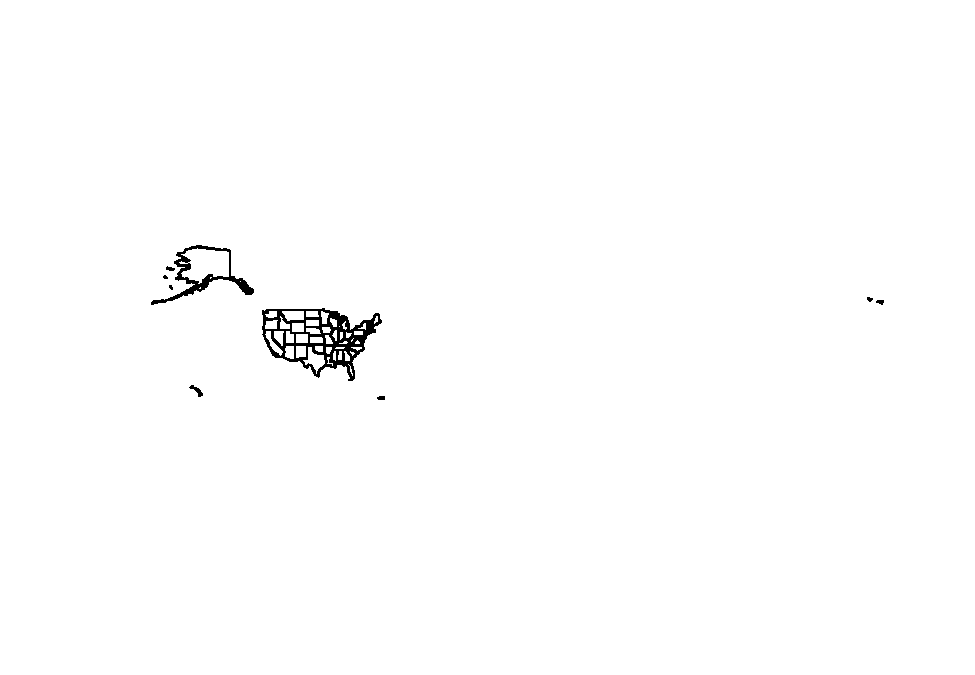
\includegraphics{lab3_patch_design_files/figure-latex/unnamed-chunk-2-1.pdf}

\begin{Shaded}
\begin{Highlighting}[]
\CommentTok{# What are the unique entries in the field, NAME?}
\KeywordTok{unique}\NormalTok{(uss}\OperatorTok{$}\NormalTok{NAME)}

\CommentTok{# We can project these data to match the NLCD data coordinate reference system (Albers, also known as NAD83 / Albers NorthAm). Fed Data R package returns NLCD data in a different CRS.}
\CommentTok{# Here's the CRS info for the CRS that FedData returns for NLCD (Pseudo Mercator: https://epsg.io/3857)}
\NormalTok{merc.proj <-}\StringTok{ }\KeywordTok{CRS}\NormalTok{(}\StringTok{"+proj=merc +a=6378137 +b=6378137 +lat_ts=0 +lon_0=0 +x_0=0 +y_0=0 +k=1 +units=m +nadgrids=@null +wktext +no_defs"}\NormalTok{)}
\CommentTok{# Here's the CRS info for CONUS North America Albers Equal Area Conic (https://epsg.io/5070)}
\NormalTok{us.aea.proj <-}\StringTok{ }\KeywordTok{CRS}\NormalTok{(}\StringTok{"+proj=aea +lat_1=29.5 +lat_2=45.5 +lat_0=23 +lon_0=-96 +x_0=0 +y_0=0 +ellps=GRS80 +datum=NAD83 +units=m +no_defs"}\NormalTok{)}

\CommentTok{# First let's make a shapefile of just Oregon from the entire US shapefile:}
\NormalTok{or <-}\StringTok{ }\NormalTok{uss[uss}\OperatorTok{$}\NormalTok{NAME }\OperatorTok{==}\StringTok{"Oregon"}\NormalTok{,] }

\CommentTok{# Plot Oregon}
\KeywordTok{plot}\NormalTok{(or)}
\end{Highlighting}
\end{Shaded}

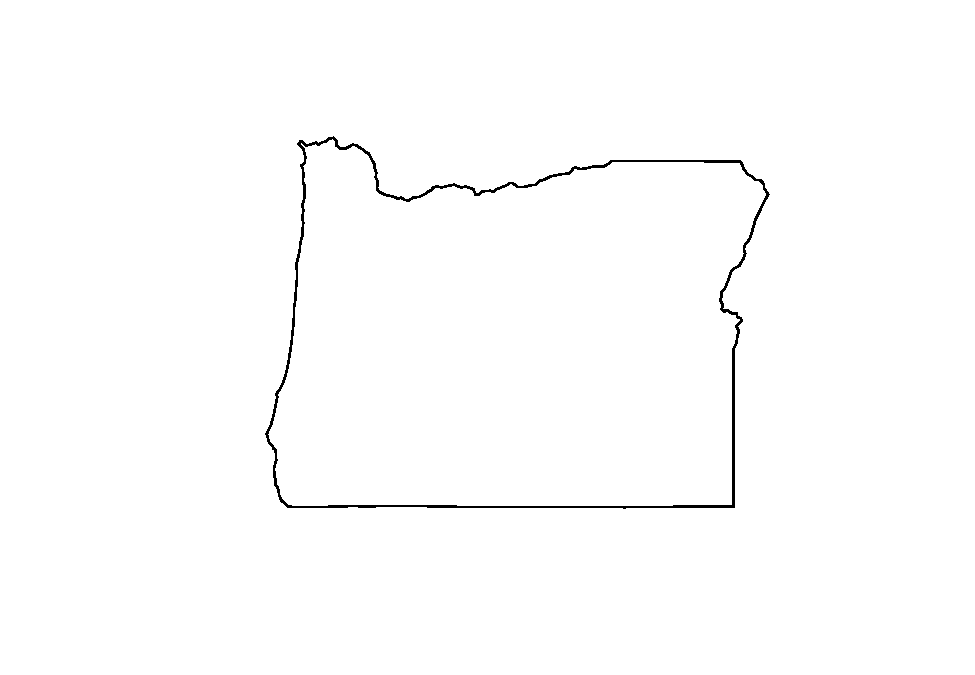
\includegraphics{lab3_patch_design_files/figure-latex/unnamed-chunk-2-2.pdf}

\begin{Shaded}
\begin{Highlighting}[]
\CommentTok{# Practice projecting, and plot again}
\NormalTok{or1<-}\KeywordTok{spTransform}\NormalTok{(or, us.aea.proj)}
\KeywordTok{plot}\NormalTok{(or1)}
\end{Highlighting}
\end{Shaded}

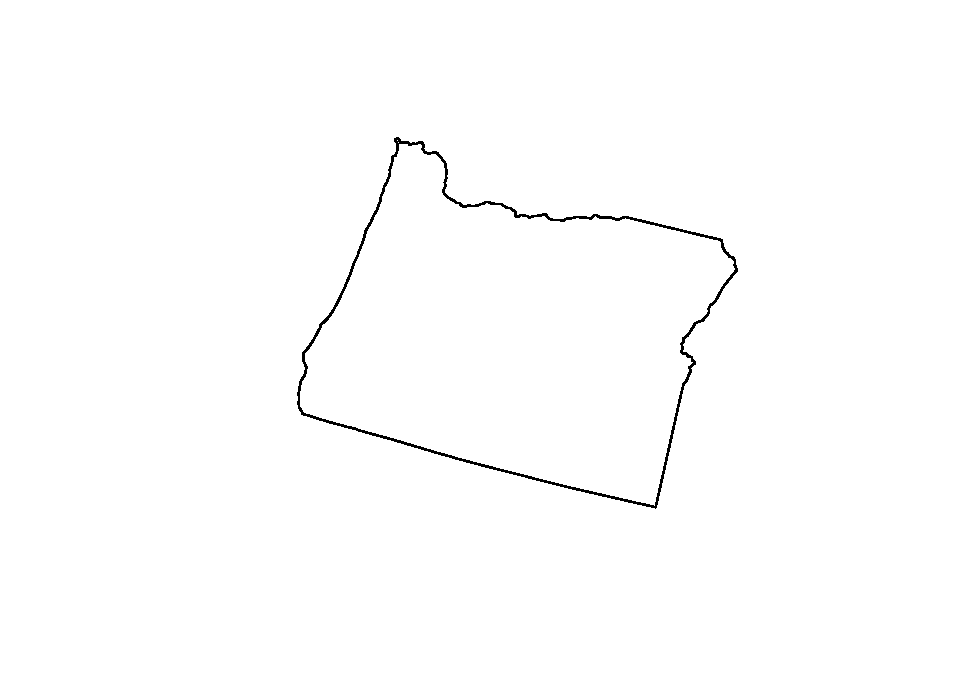
\includegraphics{lab3_patch_design_files/figure-latex/unnamed-chunk-2-3.pdf}

\begin{Shaded}
\begin{Highlighting}[]
\CommentTok{# Supposed you decide to use a rectangle instead of the Oregon polygon boundary.}
\CommentTok{# Refer to the extent (min and max x and y) of the shapefile, "or1"}
\KeywordTok{summary}\NormalTok{(or1)}
\NormalTok{or2 <-}\StringTok{ }\KeywordTok{polygon_from_extent}\NormalTok{(raster}\OperatorTok{::}\KeywordTok{extent}\NormalTok{(}\OperatorTok{-}\DecValTok{2294351}\NormalTok{,}\OperatorTok{-}\DecValTok{1584307}\NormalTok{,}\DecValTok{2301475}\NormalTok{,}\DecValTok{2899476}\NormalTok{), }\DataTypeTok{proj4string=}\StringTok{'+proj=aea +lat_1=29.5 +lat_2=45.5 +lat_0=23 +lon_0=-96 +x_0=0 +y_0=0 +ellps=GRS80 +datum=NAD83 +units=m +no_defs'}\NormalTok{)}

\CommentTok{# See how the or2 outlines to the polygon, "or1"}
\KeywordTok{plot}\NormalTok{(or2)}
\KeywordTok{plot}\NormalTok{(or1,}\DataTypeTok{add=}\NormalTok{T, }\DataTypeTok{col=}\StringTok{"blue"}\NormalTok{)}
\end{Highlighting}
\end{Shaded}

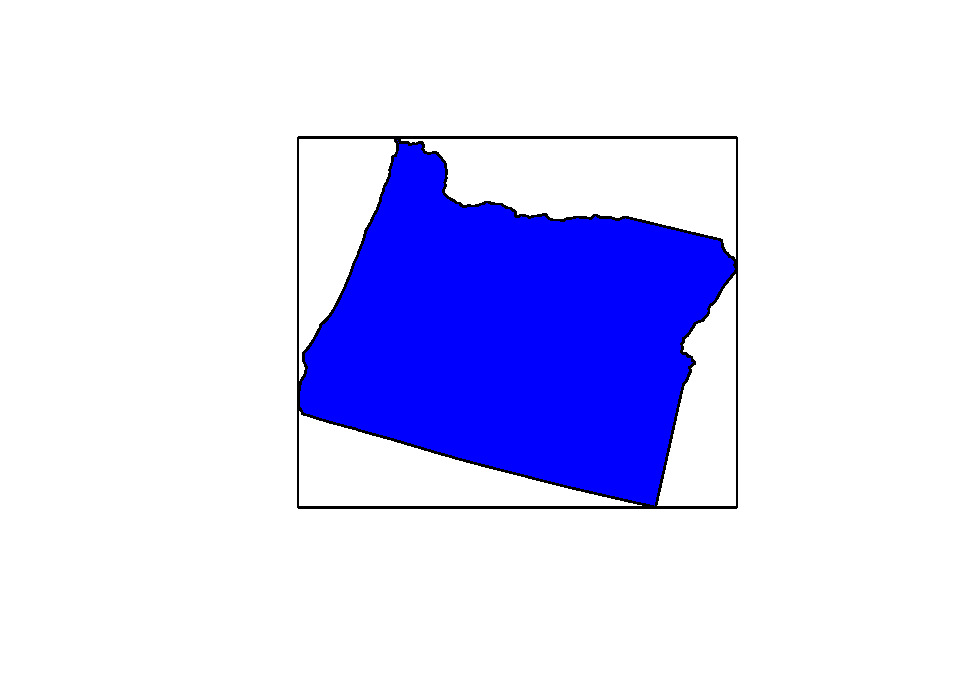
\includegraphics{lab3_patch_design_files/figure-latex/unnamed-chunk-2-4.pdf}
Depending on your computer, these polygons will still be too big to
extract NLCD quickly (when I run it on my laptop it takes about 5 mins,
so you could try it but it may get hung up if you are knitting to PDF).
Let's try a smaller extent. If you wanted to subset out just a portion
of Oregon, you could select 1 wildlife management unit. Here is a map of
OR Fish \& Wildlife Units:
\url{https://www.dfw.state.or.us/resources/hunting/big_game/units/bigmap.asp}.
\href{https://www.dfw.state.or.us/resources/hunting/big_game/units/images/bigmapa2.gif}{\includegraphics{bigmapa2.gif}}

Repeat the same process as above with Oregon:

\begin{Shaded}
\begin{Highlighting}[]
\ControlFlowTok{if}\NormalTok{(}\OperatorTok{!}\StringTok{ }\KeywordTok{file.exists}\NormalTok{(}\StringTok{'mgmt.zip'}\NormalTok{))\{}
 \KeywordTok{download.file}\NormalTok{(}\StringTok{"https://nrimp.dfw.state.or.us/web%20stores/data%20libraries/files/ODFW/ODFW_805_5_wildlife_mgmt_units.zip"}\NormalTok{,}\DataTypeTok{dest=}\KeywordTok{file.path}\NormalTok{(data_path,}\StringTok{"mgmt.zip"}\NormalTok{), }\DataTypeTok{mode=}\StringTok{"wb"}\NormalTok{) }
\NormalTok{\}}
\KeywordTok{unzip}\NormalTok{ (}\KeywordTok{file.path}\NormalTok{(data_path,}\StringTok{"mgmt.zip"}\NormalTok{), }\DataTypeTok{exdir =}\NormalTok{ data_path)}
\NormalTok{mgmt<-}\KeywordTok{readOGR}\NormalTok{(}\KeywordTok{file.path}\NormalTok{(data_path,}\StringTok{"wmu24poly.shp"}\NormalTok{))}

\KeywordTok{summary}\NormalTok{(mgmt) }\CommentTok{# Its CRS is lcc (Lambert Conformal Conic: https://proj.org/operations/projections/lcc.html)}
\NormalTok{lcc.proj<-}\KeywordTok{CRS}\NormalTok{(}\StringTok{"+proj=lcc +lat_0=41.75 +lon_0=-120.5 +lat_1=43 +lat_2=45.5 +x_0=400000 +y_0=0 +datum=NAD83 +units=ft +no_defs"}\NormalTok{)}

\CommentTok{# Project mgmt into the lcc projection from the Oregon NLCD 2011 (see below)}
\NormalTok{mgmt1<-}\KeywordTok{spTransform}\NormalTok{(mgmt, lcc.proj)}

\KeywordTok{head}\NormalTok{(mgmt1)}
\KeywordTok{unique}\NormalTok{(mgmt1}\OperatorTok{$}\NormalTok{UNIT_NAME)}
\CommentTok{# Select the HOOD Management Unit (where Mount Hood is).}
\NormalTok{hood <-}\StringTok{ }\NormalTok{mgmt1[mgmt}\OperatorTok{$}\NormalTok{UNIT_NAME }\OperatorTok{==}\StringTok{"HOOD"}\NormalTok{,] }
\CommentTok{## See where it's located. Plotting and rendering may take a minute because these polygons are complex.}
\KeywordTok{plot}\NormalTok{(mgmt1)}
\KeywordTok{plot}\NormalTok{(hood,}\DataTypeTok{add=}\NormalTok{T,}\DataTypeTok{col=}\StringTok{"red"}\NormalTok{)}
\end{Highlighting}
\end{Shaded}

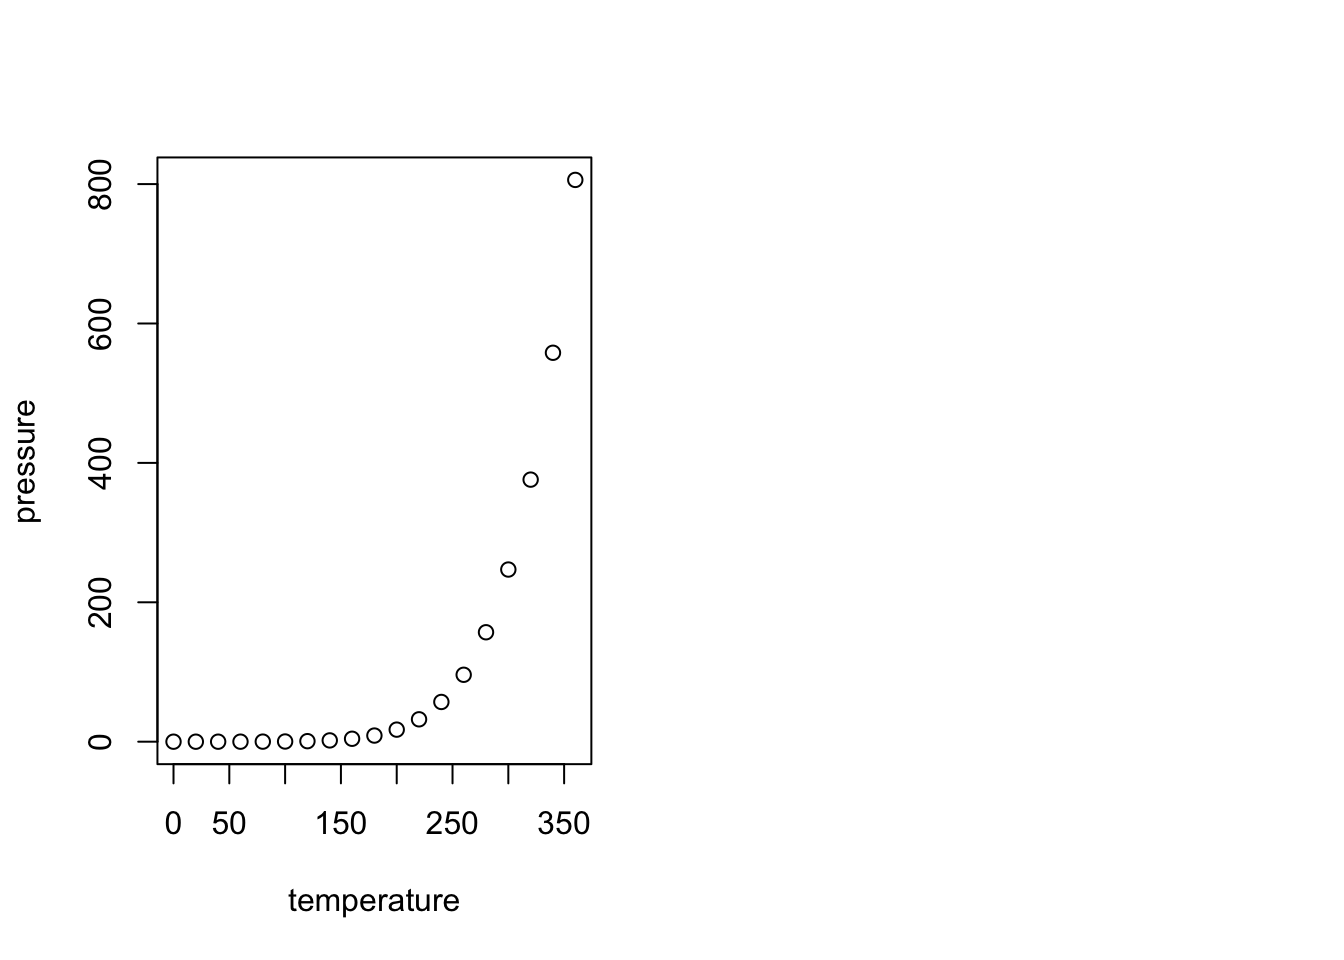
\includegraphics{lab3_patch_design_files/figure-latex/unnamed-chunk-3-1.pdf}

\begin{Shaded}
\begin{Highlighting}[]
\CommentTok{## Here is where you will import the Oregon NLCD directly (if the FedData package is not installing correctly), OR start using the FedData package to download the 2016 data.}

\CommentTok{## OPTION 1: Importing the Oregon 2011 NLCD data directly}
\CommentTok{## Download the 2011 Oregon NLCD (54 MB) - may take a few mins}
\CommentTok{## Download the Oregon NLCD (54 MB) - uncomment below}
\CommentTok{# if(! file.exists('or_nlcd.zip'))\{}
\CommentTok{# download.file("http://oe.oregonexplorer.info/ExternalContent/SpatialDataforDownload/OR_NLCD_2011.zip", dest=file.path(data_path,"or_nlcd.zip"), mode="wb")}
\CommentTok{# \}}
\CommentTok{# unzip (file.path(data_path,"or_nlcd.zip"), exdir = data_path)}
\CommentTok{# or_nlcd <- raster(file.path(data_path,"./OR_NLCD_2011/nlcd_or_20111" ))}
\CommentTok{# save.image("lab3.RData")}
\CommentTok{# }
\CommentTok{# # Take a look at or_nlcd from 2011 - it is projected in lcc}
\CommentTok{# or_nlcd}
\CommentTok{# }
\CommentTok{# # Crop or_nlcd by hood1}
\CommentTok{# hood_nlcd<-crop(or_nlcd, extent(hood))}
\CommentTok{# hood_nlcd <- mask(x = hood_nlcd, mask = hood)}

\CommentTok{# plot(hood_nlcd)}
\CommentTok{# plot(hood,add=TRUE, lwd=2, border='white')}

\CommentTok{## Uncomment to output a raster as a tif}
\NormalTok{?writeRaster}
\CommentTok{#writeRaster(raster, "raster.tif")}

\CommentTok{## OPTION 2 (uncomment below): Use the get_nlcd command from FedData to extract the NLCD data for this management unit. FedData does the cropping automatically using a shapefile or raster for "template". If you run into errors you may need to check what the projection of hood_nlcd is.}
\CommentTok{# ?get_nlcd}
\CommentTok{# }
\CommentTok{# hood_nlcd<-get_nlcd(}
\CommentTok{#   template = hood,}
\CommentTok{#   label="Hood",}
\CommentTok{#   year = 2016,}
\CommentTok{#   dataset = "Land_Cover",}
\CommentTok{#   extraction.dir = paste0(data_path, "/FedData/"),}
\CommentTok{# )}
\CommentTok{# hood_nlcd}

\CommentTok{# plot(hood_nlcd)}
\CommentTok{# plot(hood,add=TRUE, lwd=2, border='white')}
\end{Highlighting}
\end{Shaded}

Now work with the \texttt{landscapemetrics} R package to compute
different patch and landscape statistics.

\begin{Shaded}
\begin{Highlighting}[]
\CommentTok{## Make a plot of the Hood NLCD data - this renders a map of the NLCD raster. It may take a few mins to render. Then check to see if the input data is suitable for computing patch metrics}
 
\CommentTok{#show_landscape(hood_nlcd)}
\CommentTok{#check_landscape(hood_nlcd)}
\end{Highlighting}
\end{Shaded}

You could proceed to calculate metrics for all different land cover
classes (this would take a while). Instead, suppose you are interested
in the metrics of ``forested'' patches in this landscape. First,
reclassify into ``forest'' and ``nonforest''. You need to determine what
the cover types are:

\begin{Shaded}
\begin{Highlighting}[]
\CommentTok{#unique(hood_nlcd)}
\CommentTok{## Look here at the "Class/Value" to figure out which cover type(s) you want: https://www.mrlc.gov/data/legends/national-land-cover-database-2016-nlcd2016-legend. For example, evergreen is 42. However, there are other forest cover types as well. Determine how to make the raster "all forest" not just evergreen. Umncomment below:}
\CommentTok{#hood_for <- hood_nlcd}
\CommentTok{#hood_for[hood_for < 41] <- 0 # make everything below 41 zero}
\CommentTok{#plot(hood_for)}
\CommentTok{#hood_for[hood_for > 43] <- 0 # make everything above 43 zero}
\CommentTok{#plot(hood_for)}
\CommentTok{#unique(hood_for)}
\CommentTok{## Assign 1 value (1) to forest.}
\CommentTok{#hood_for[hood_for == 41 | hood_for == 42 | hood_for == 43] <- 1}
\CommentTok{#show_landscape(hood_for)}

\CommentTok{## The code below follows part of this vignette: https://r-spatialecology.github.io/landscapemetrics/articles/articles/utility.html - check it out for more context and if you would like to try other commands not covered here.}

\CommentTok{## Check to see if the input data is suitable for computing patch metrics}
\CommentTok{#check_landscape(hood_for)}

\CommentTok{## Look at the distinct patches for this landscape}
\CommentTok{#show_patches(hood_for) }

\CommentTok{## Show patches of each class (we have 2 classes: 0 for non-forest and 1 for forest)}
\CommentTok{#show_patches(hood_for, class = "all", labels = FALSE)}

\CommentTok{## At the patch level, compute patch metrics}
\CommentTok{#hood_metrics <- calculate_lsm(hood_for, what = "patch")}

\CommentTok{## Look at the different types of metrics at the patch level. Note that you can compute these metrics at the patch, landscape, or class levels.}
\CommentTok{#list_lsm(level='patch')}

\CommentTok{## Determine if any patch metrics are correlated}
\CommentTok{#show_correlation(hood_metrics, method = "pearson")}
\end{Highlighting}
\end{Shaded}

\#\#\#QUESTION 1: How do the 12 patch metrics from
\texttt{landscapemetrics} help you understand how an organism interacts
with its environment? For 3 metrics of your choice, explain in 1-2
sentences what the metric tells us about an organism's interaction with
its environment. Feel free to use examples. Refer to the
\emph{list\_lsm()} results above. You may also want to refer to the
FRAGSTATS documentation for more in-depth coverage (warning: this is a
large document, I suggest searching for the patch metric term. Page 77
contains the start of the ``metrics'' discussion, but page 92 contains a
condensed table):
\url{https://www.umass.edu/landeco/research/fragstats/documents/fragstats_documents.html}

\#\#\#QUESTION 2: Repeat the process above, but select a different
management unit than Hood. Compare your other management unit patch
metrics with the ones for Hood Management Area. Briefly, how do the
patch metrics for Forested areas and non-Forested areas compare between
the two management areas? Optional: make some plots showing the
statistical distributions of patch metrics across the two areas (e.g., a
histogram of patch area, by class, by management unit).

\hypertarget{part-2-study-design}{%
\subsection{Part 2: Study Design}\label{part-2-study-design}}

You decide to study the interactions between Spotted Owls and Barred
Owls in Oregon forests (do a little internet searching to understand why
studying these 2 species together is important, and what their habitat
requirements are).

\#\#\#QUESTION 3. Use GBIF data to generate a map showing ``recent''
point locations of each of these species (as different symbols and/or
different colors), overlain on top of the 2 forest rasters you created
above. Justify the timeframe you chose for the occurrences. Make 2 maps,
one for each management unit with the points overlaid on top of the
forest raster. Include a legend, scalebar (with units), and north arrow
for your maps. You may want to reference Lab 2 for additional code.

\#\#\#QUESTION 4. If you had unlimited resources, describe how you would
sample the 2 management units to obtain new occurrence data next year
for both species. Are there specific forest attributes that would be
helpful to know in addition to just ``forest vs.~non-forest''? Use
terminology we covered in Lecture and Discussion about sampling.

\emph{Some other potentially helpful code below:}

\texttt{gbif}: Extract out just points from Oregon (or some extent):
\url{http://www.inside-r.org/packages/cran/dismo/docs/rgbif}. There are
2 ways of extracting out the points:

The commands, \texttt{drawExtent} and \texttt{extent} are both ways to
specify the extent of data in \texttt{gbif()}

\texttt{drawExtent} is in the raster package:
\url{http://www.inside-r.org/packages/cran/raster/docs/drawExtent}. You
have to have plotted a map first (and then click on it). This won't be
possible if you're running a script via job submission on HPCC. You can
also use \texttt{extent}, also in the raster package, to define
boundaries:
\url{http://www.inside-r.org/packages/cran/raster/docs/extent}

\hypertarget{homework-in-preparation-for-lab-4}{%
\subsection{Homework in preparation for Lab
4:}\label{homework-in-preparation-for-lab-4}}

In Lab 4 we will introduce GitHub, a versioning program helpful for
collaborating and tracking changes in code. You can think of it as a
Google Docs version for tracking code changes (you can also use it with
text). If you are familiar with GitHub, no need to go over the
following, but if you are not familiar, please work through the
following tutorials {[}personally, I use the Desktop version but any
version will work{]}:

At a minimum, please complete this first short tutorial ahead of Lab 4:
1. Command line version:
\url{https://guides.github.com/activities/hello-world/}

Other versions: 2. Desktop version:
\url{https://help.github.com/desktop/guides/getting-started-with-github-desktop/}

\begin{enumerate}
\def\labelenumi{\arabic{enumi}.}
\setcounter{enumi}{2}
\tightlist
\item
  via RStudio: \url{http://happygitwithr.com/rstudio-git-github.html}
  and/or
  \url{https://support.rstudio.com/hc/en-us/articles/200532077-Version-Control-with-Git-and-SVN}
\end{enumerate}

This work is licensed under a Licensed under CC-BY 4.0 2020 by Phoebe
Zarnetske.

\end{document}
